\section{Motivation and approach\label{section:deductive-motivation}}

Building adequate, complete and consistent process models is not necessarily an easy task. Flawed models can have dreadful consequences in safety-critical areas. The recent usage of process modeling to improve medical safety provides a good example of such area \cite{Clarke:2008, Grando:2009, Damas:2011}; models there should be as free of errors as possible. Techniques should therefore be available for helping building them, in particular for systematically detecting and fixing severe flaws.

An typical analysis technique that comes in mind is \emph{model checking} \cite{Clarke:1989}. Model-checking would allow verifying that a given safety property is satisfied in all process instances. Other kinds of analysis on process models are discussed in \cite{Damas:2011}; this includes checking the satisfiability of guards; verifying that temporal constraints are met; detecting inaccurate process decisions; and so on. This kind of check should be performed ahead of process enactment.

Verification techniques require providing a formal semantics to the process models. As our guarded hMSCs are an extension of hMSCs, providing them a trace semantics appears natural. This choice is also motivated by the accessibility to stakeholders; trace semantics can indeed be rephrased as the temporal occurrence of tasks. Moreover, providing a trace semantics to g-hMSCs enables reusing LTS tools and techniques \cite{Magee:1999, Giannakopoulou:2003}.

\begin{figure}\centering
\scalebox{0.6}{
  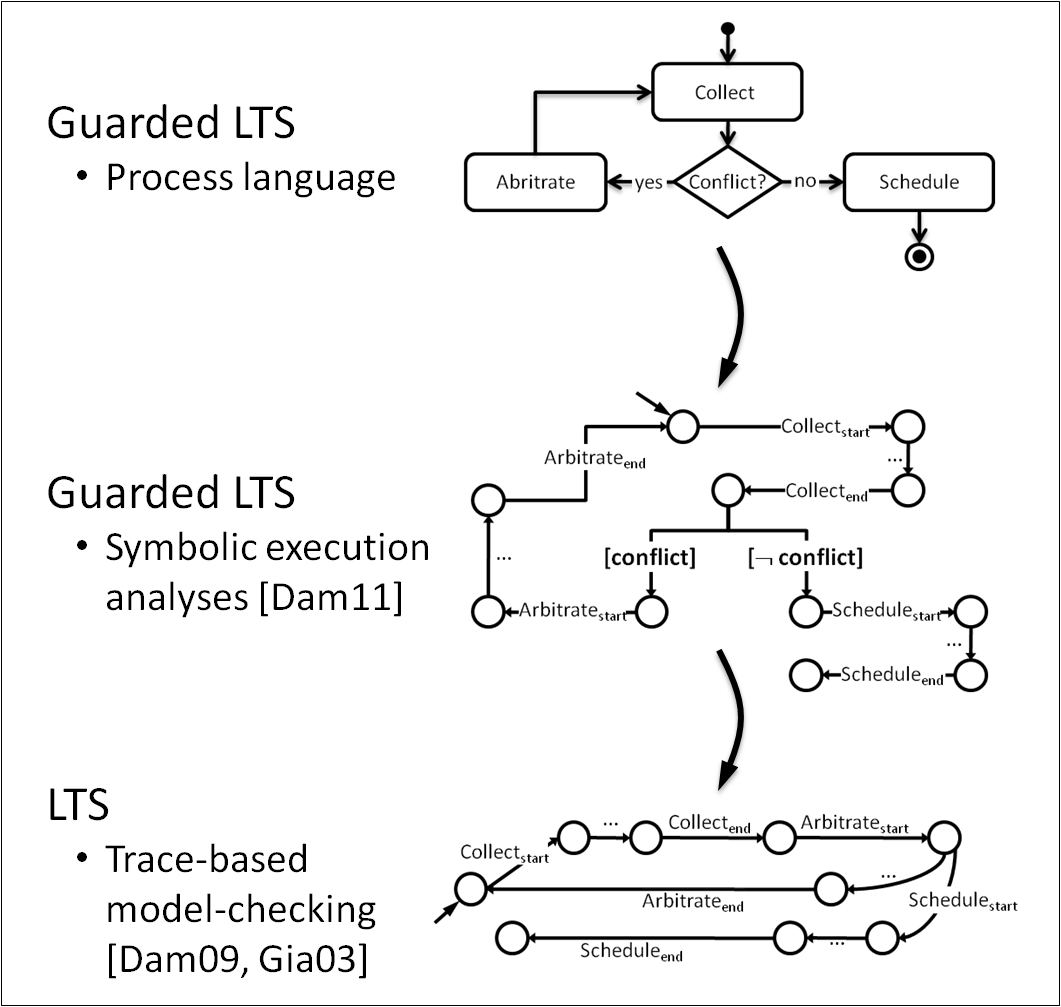
\includegraphics[trim=2mm 2mm 2mm 2mm, clip]{src/3-deductive/images/chapter-overview}
}
\caption{Guarded LTS as an intermediate level between g-hMSC and LTS.\label{image:deductive-chapter-overview}}
\end{figure}

Note that we will only consider the traces of a process globally, that is, as sequences of events seen by an external observer. In other words, even if our process models provide a multi-agent view through the message sequence charts, we will not consider agent state machines in isolation. Remember that the aim of process modeling is \emph{not} to specify valid executions of the agents themselve, but valid control flow of their tasks. The hypothese of strong sequential composition of g-hMSC tasks and the introduction of the special events $T_{start}$ and $T_{end}$ effectively enforces this.

Instead of directly rewriting guarded hMSC as LTS, however, we will use an intermediate level through guarded labeled transition systems (g-LTS). Roughly, a g-LTS is a transition system with guards or events on transitions. It is mainly introduced for providing a structured form of LTS that avoids state explosion. It is therefore easier to understand and facilitates code generation needed for process enactment. 

Figure~\ref{image:deductive-chapter-overview} illustrates the three abstraction levels provided by g-hMSC, g-LTS and LTS. Analyzes about guards, temporal constraints, etc. are performed at the g-LTS level. They rely on an generalization of the symbolic execution algorithm used to decorate a LTS with assertions on fluents, discussed in Section \ref{section:background-fluents}. For details about analyzes at the g-LTS level, see \cite{Damas:2011}. Trace-based model-checking can be performed at the LTS level, using existing tools such as LTSA \cite{Magee:1999}. An integrated approach that brings model-checking at the g-hMSC and g-LTS levels is also detailed in Section \ref{section:tool-model-checker}.

The two synthesis algorithms for rewriting a guarded hMSC to a guarded LTS then to a LTS are detailed in Section \ref{section:deductive-glts-to-lts}. Section \ref{section:deductive-glts} will first introduce guarded LTSs formally; it also provides a few operators to manipulate them.
